\documentclass[a4paper,11pt]{article}
\usepackage{amsmath}
\usepackage{fancyhdr}
\usepackage{graphicx}
\usepackage{url}
\usepackage{float}
\usepackage{amsmath}
\usepackage[margin=1in]{geometry}

\newcommand{\suchthat}{\;\ifnum\currentgrouptype=16 \middle\fi|\;}
%\usepackage[top=.6in, bottom=.8in, left=.8in, right=.8in]{geometry}

% \floatstyle{boxed}
% \restylefloat{figure}
%==== Insert cool image between title and authors ====%
\title{Using 3D Models and Computer Vision Algorithms to \\ Implement Monte Carlo Localization}
\author{ \\[7in]  John Allard, Alex Rich \\ 2014 Summer Computer Science REU, Harvey Mudd College\thanks{Funded By The National Science Foundation and mentored by Professor Zachary Dodds}}
%\date{July 6th, 2014 \\}

\begin{document}

% ==== Title Page ==== %
  \maketitle   
  \newpage  
  
% ==== Table Of Contents ==== %
  \tableofcontents
  \newpage

  % ==  Paper Abstract   == %
  \begin{abstract}  
  Our research group attempts to implement the Monte Carlo Localization algorithm using a 3D model of an environment and a stream of images from a robot in that environment. This entails the use of various computer vision algorithms to find and compare features between the image feed and our 3D model. The objectives of this project are to be able to localize a general actor in any 3D modeled environment quickly and accurately. This paper outlines the process that our research group has undertaken to accomplish this task and an analysis of our resulting program. 
  \end{abstract}
  
















%====================================%
%===== Section 1, Introduction ===== %
%====================================%
  \section{Introduction} 

  \subsection{Project Overview}
  The Monte Carlo Localization (MCL) algorithm has been used in the past\footnote{ Dieter Fox, et al. Carnegie Mellon University, University of Bonn.} to successfully localize robots using 2D maps of an environment and a stream of range sensor information. Our goal was to build off of these successes and implement a similar algorithm using a 3D map and color images from the robot as sensor data. The end goal of this project was to be able to place a robot anywhere inside of a mapped environment, have our program quickly and reliably localize the robot, then continue to localize the robot as it moves around the environment in attempt of accomplishing its programmed goals (fetching coffee, cleaning the floor, etc).

 We chose to implement the MCL algorithm using 3D models and a live image-feed from the robot because it appears that this will be a common goal for robots to be able to perform in the near future. 3D models of an environment might be difficult to curently obtain, but they are constantly getting easier and cheaper to create. Our camera was donated by a new start-up company called Matterport, as companies like this grow we should see a proliferation of 3D-imaging cameras accompanied by a general decrease in price and increase in scan-quality. The reason we decided to use a camera as a sensor device instead of a range sensor is because cameras have continued following the trend in recent years of becoming cheaper and more portable, and the extra information present in an image compared to a set of range sensor data could make the localization process easier and more robust. The combination of these two trends suggests that the need for research related to localizing a robot using 3D models and image data is going to grow in the upcoming years, which is why we decided to undertake on this project.

 \subsection{About}
 This project was undertaken by Alex Rich and John Allard during the Summer of 2014 at Harvey Mudd College, under the mentorship of Professor Zach Dodds. Our project was part of the Harvey Mudd Computer Science REU, with funding that originated from the National Science Fondation. The website/blog that organizes everything related to this project (including our code repository, code documentation, and research artifacts) is hosted here : \\
\texttt{https://jhallard.github.io/3DLocalization}

\newpage

% ==   1.1 Process Overview  == %
  \section{Monte Carlo Localization Process Overview}
%  \emph{This section is for those unfamiliar with the Monte Carlo Localization algorithm.}

The overall process of having an actor\footnote{An actor is any device that has sensors and can move around an environment, e.g. a robot.} localize itself in an environment via the MCL algorithm is comprised of many steps. A general outline of these steps is given below.
\subsection{Pre-Localization}
 These are the requirements that must be satisfied to begin the MCL algorithm.
  \begin{enumerate}
  \item A map of the environment needs to be imported or constructed. 
  \item Some type of quantifiable features present in the map that can be detected with a sensor on the robot must be chosen (image features, range data, etc). This enables a comparison between sensor readings from the actor and the expected sensor readings from different places in the map.
  \item This step is optional.  Features from the map are computed from many different reference points and are stored for use during the localization attempt. This significantly narrows the set of locations that the robot can be determined to be at compared to generating feature data at run-time, but it reduces the computational resources needed significantly and allows one to simply look up the data in a map or container as opposed to computing it in real-time. Pre-computing features also significantly reduces the complexity of the localization source code.
  \end{enumerate}
\subsection{During Localization}
  The MCL algorithm iterates through a series of steps to determine the location of an actor. Each step can be implemented in a variety of different ways.
  \begin{enumerate}
  \item An actor is placed somewhere in the environment, and some number of guesses as to where it might be are randomly generated.\footnote{The uniformity of this distribution depends on the user's knowledge of the actor's initial location.} These `guesses' we will call particles, and each particle is a data structure that contains information about its own current perspective in the environment and the sensor data it would expect to read from that perspective.
  \item The program compares the current sensor readings from the actor to the expected sensor readings for each particle, and assigns a weight to each particle based on how strongly the readings correspond to one another.
  \item A distribution is created according to the grouping and weighting of particles active in the program. The more heavily weighted a particle is, the higher probability it or one of its close neighbors will be sampled from our distribution during the next step.
  \item A new set of particles are sampled from this distibution, as well as a small amount are sampled from a uniform distribution across the map. After this step the total number of particles in the program is the same as in the last step.
  \item The actor is moved to a new point in the environment via some movement command from the actor control program. Each particle has its perspective updated according to the same commands, plus some statistical error from the uncertainty in the actor's movements. The expected sensor readings for each particle are also updated to correspond to its new perspective of the environment.
  \item Steps 2-4 are repeated until we recieve an \texttt{end-program} command or we otherwise lose contact with the actor. As long as there is a connection our program will attempt to compute the actors location and relay this data to the actor. The general idea is as we weigh and resample the particles, the locations of the particles should converge on the actor's location in the environment.
  \end{enumerate} 
  
 The power of this algorithm comes from a few key characterstics. 
\begin{itemize}
 \item The algorithm is very general and leaves a large amount of the implementation details for the user to decide. As was stated before, this algorithm has been used in the past with both laser and sonar range data and a 2D map of an environment, in our case it was used with images from the robot and a 3D model of the environment. This algorithm is applicabile to virtually any type of sensor data, as long as this data can be compared to the expected sensor readings that various places in a map. 
 \item Secondly, from the mobility of the particles. When the actor moves, the particles move, and thus they store the probability that the actor has traveled in the path that the particle has taken. Over time, impossible paths will cause incorrect particles to be removed from the current set of guesses, leaving room for better guesses to take their place. This results in the gradual merging of particles in space to the correct location.
\end{itemize}

\newpage














%=====================================%
%===== Section 2, 3D Map Building ====%
%=====================================%
  \section{Building the 3D Map}
   \subsection{Overview}
  Our research team used three dimensional models to serve as maps of the actor's environment for the localization process. These models were fully textured, high-quality scans of a room or series of rooms and hallways. The 3D maps were built using a Matterport 3D imaging camera donated to our research group by Matterport Inc. This camera is attached to the top of a tripod and placed somewhere in an enclosed environment, it then uses an internal motor to rotate 360 degrees and take a scan of the space using both an RGB camera and laser-range sensors. Subsequent scans are merged with the existing model, allowing one to walk the camera around a space and progressively build a larger and more detailed model.

   \begin{figure}[h!]
   \centering
     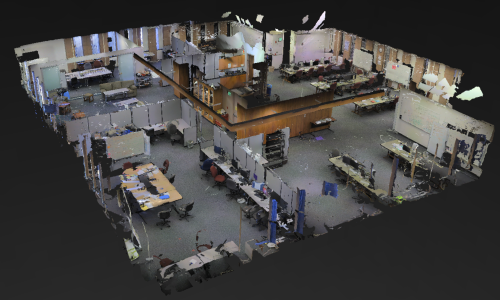
\includegraphics[height=1.9in,width=4.9in,angle=0]{../Artifacts/rp1}
   \caption{3D model of the Sprague environment.}
  \end{figure}
  
  \subsection{Taking the Scans}
 Our team built models of various places on the Harvey Mudd campus, but the main environment that we wished to localize an actor in was the 2nd floor of the Sprague building, where we work. We took 42 scans of this space (Seen in \emph{Figure 1}), a roughly 3500 sqft floor consisting of 7-8 rooms and a large amount of non-static objects, such as chairs, laptops, and people. The Matterport software allows up-to 100 separate scans to form a single model, and the software bundled with the camera automatically merges these scans into one textured mesh. The software also automatically converts the data to a \texttt{Wavefront .obj} file format for viewing on their site. We were then able to download this file to use it in our own 3D model viewers. 

  \subsection{Filling In the Gaps}
  Our model was inevitably left with gaps from places that were obstructed from the view of our camera. To help improve the overall quality of our map we used the Meshlab software. This allowed us to remove disconnected pieces, remove unreferenced vertices, and smoothen out some jagged areas. on top of this, we rendered the background color pink to allow us to single out features on these areas and remove them from the program. 
  
  \newpage



















 %==================================================================%
 %===== Section 3, Creating a Database of Images from the Map ===== %
 %==================================================================%
   \section{Creating a Database of Images from the Map}
  Our goal is to use computer vision algorithms that perform comparisons between 2D images, which meant that we had to represent our 3D map in 2D for our feature matching algorithms to work properly. To represent our 3D map as 2D information, we decided to render images from thousands of different perspectives within our map.

  \begin{figure}[h!]
   \centering
     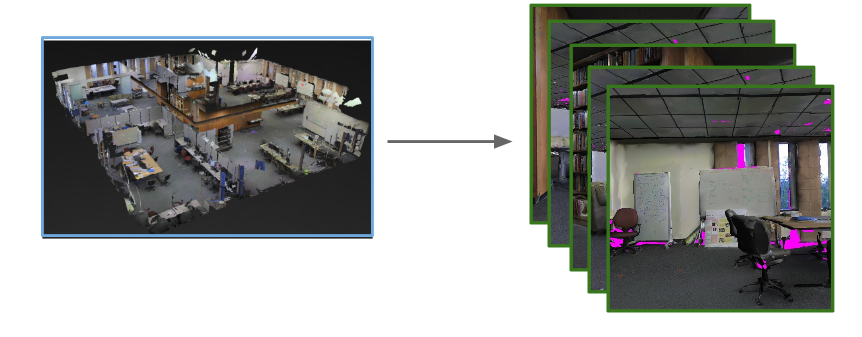
\includegraphics[height=2.1in,width=5.3in,angle=0]{../Artifacts/RenderImages}
   \caption{Turning a 3D model into 2D images.}
  \end{figure}
 
  There are of course many different ways to decide which subset of points within the map will be chosen to render images from. The method our group used is outlined below.

  \begin{enumerate}
  \item Establish a bounding box around our map.
  \item Define a plane, bounded by the box defined above, that sits above and parallel to the x-y plane of our map at some constant z height.
  \item Define the a grid of a certain density on this plane (e.g. \texttt{[0.2 x 0.2]} grid squares).
  \item Go to each grid intersection and render images from \texttt{n} perspectives, where \texttt{n} is some number that cleanly divides 360. Our group used \texttt{n = 8}, rendering pictures from an angle of \texttt{[0, 45, 90, ..., 315, 360]} degrees in the x-y plane at each grid intersection.
  \item Name the images according to their location in the map and store them for later use.
  \end{enumerate} 


  This process allows us to turn our 3D model into a catalogued database of 2D images from a large amount of places within our model. From here we can use existing computer vision related algorithms (SURF, SIFT, ORB, etc.) to do the keypoint detection and feature description needed to match images with one another.

 \newpage






















%=======================================================%
%===== Section 4, Computing Features from the Map ===== %
%=======================================================%
  \section{Computing Features from the Map}
After generating a database of images and labeling them according to their perspective in the environment, we had to go through and compute various types of image features from each one. This is done before localization because computing features is a computationally intensive process, and doing so during runtime significantly slows down the localization process. The information catalogued during this stage is loaded during the boot phase of the localization program.

  \subsection{Types of Features}
There are a variety of features that can be used when describing an image. In its current state, the project uses extracted SURF features as well as grayscale and black and white images.

SURF (Speeded Up Robust Features) is a feature detection algorithm that detects similar features as SIFT (Scale-Invariant Feature Transform). SURF detects interesting keypoints in an image in a manner that is a bit quicker than some competing algorithms such as SIFT, but it also lacks some nice properties like scale invariance. Using OpenCV, we can detect these points, describe them as features, save these descriptions, and eventually compare these features with ones computed from the robot during the localization process.

The Grayscale image is a highly coarse image that simply splits an image into a grid, then computes the average intensity inside each grid square. From this image, we can compute the black and white ``above below" image. This is created by finding the average intensity of the grayscale, then determining if a square is either higher or lower than this. If a square is higher, it is colored white, otherwise it is colored black.

  \subsection{Storing the Features}
The precomputed features are stored in a yaml file. OpenCV has built in storage methods, which makes this a simple process. Because each perspective has its own file for storing keypoints|in addition to its own file for grayscale and black and white images|the filename contains the meta information about each description. The program is able to load all features and know their corresponding location and orientation by first looking inside the folder to see what perspectives are available, then load into the map.

\newpage

















%========================================%
%===== Section 5, MCL Implementation ====% 
%========================================%
  \section{Implementation}

 \subsection{Overview}
 Our implementation of the Monte Carlo Localization algorithm is contained inside of a program called \texttt{3DLocalization} \footnote{See \texttt{https://github.com/jhallard/3DLocalization/Localization}}. This program is written entirely in C++, using various open-source libraries like \texttt{OpenCV}, \texttt{ROS}, and \texttt{Boost} to aid in development. All of the data that was computed by the programs described in sections 3 and 4 of this document is used by this program. \\
 Some of the main goals when designing this program are as follows 
 \begin{itemize}
 \item Make the program relatively light-weight as to not redirect computational resources from the main robot-control program.
 \item Be able to run in the background with no user input needed after the initial starting of the program. 
 \item Impose as few restrictions on the characteristics of the actor as possible (e.g. dimensions of freedom, movement timing, wheeled vs airborne).
 \item Make the program robust to environmental changes (e.g. chairs being moved, lights being dimmed).
 \end{itemize}
  Given the time frame of our research project, completing all of the above goals would be tough. Thus we used them mostly as guidelines for our team to follow as opposed to points marking the finish line of our project.
 


 \subsection{Actor Specifications}
\begin{itemize}
\item \textbf{Overview} \\
One of the main goals for our project was to be able to localize a \emph{general} actor in a \emph{general} environment. With this in mind, we tried to limit the number of requirements we impose on the movement and control of the actor. In summary, the actor must send us data from a camera and let us know its local movement coordinates, as well as listen for its global coordinates from our localization progran. All other control aspects of the actor are up to the user to decide. We have used this program successfully with both the ARDrone quad-copters and the ICreate robots, two very different robots. In our implementation, simple point to point navigation was sufficient, however a future goal is to implement the ability to make smart paths allowing the robot to go through doors and around or over tables.

\item \textbf{Communication} \\
The following functionality must be implemented by the robot
  \begin{itemize}
  \item Send two different types of data to our program. First, it must send us images from the robot's current position. The rate at which it publishes these images is not specified, but generally faster is better. Secondly, the robot must send us it's movement commands after it performs a move. These movement commands are relative to it's local coordinate system.
  \item `Subscribe` to a single data feed from our program. This data feed will tell the robot where we currently think it is in the environment, and how confident we are in our guess.
  \item The control code for the actor must be developed separately. The user chooses which robot to use, how to move the robot, and how to connect to our program. Our program only cares about localizing a general actor in a general environment.
  \end{itemize} 
\end{itemize}


 \subsection{Command Flow}
  Below is a visual overview of our implementation of the MCL algorithm, 3DLocalization.
  \begin{figure}[h!]
   \centering
     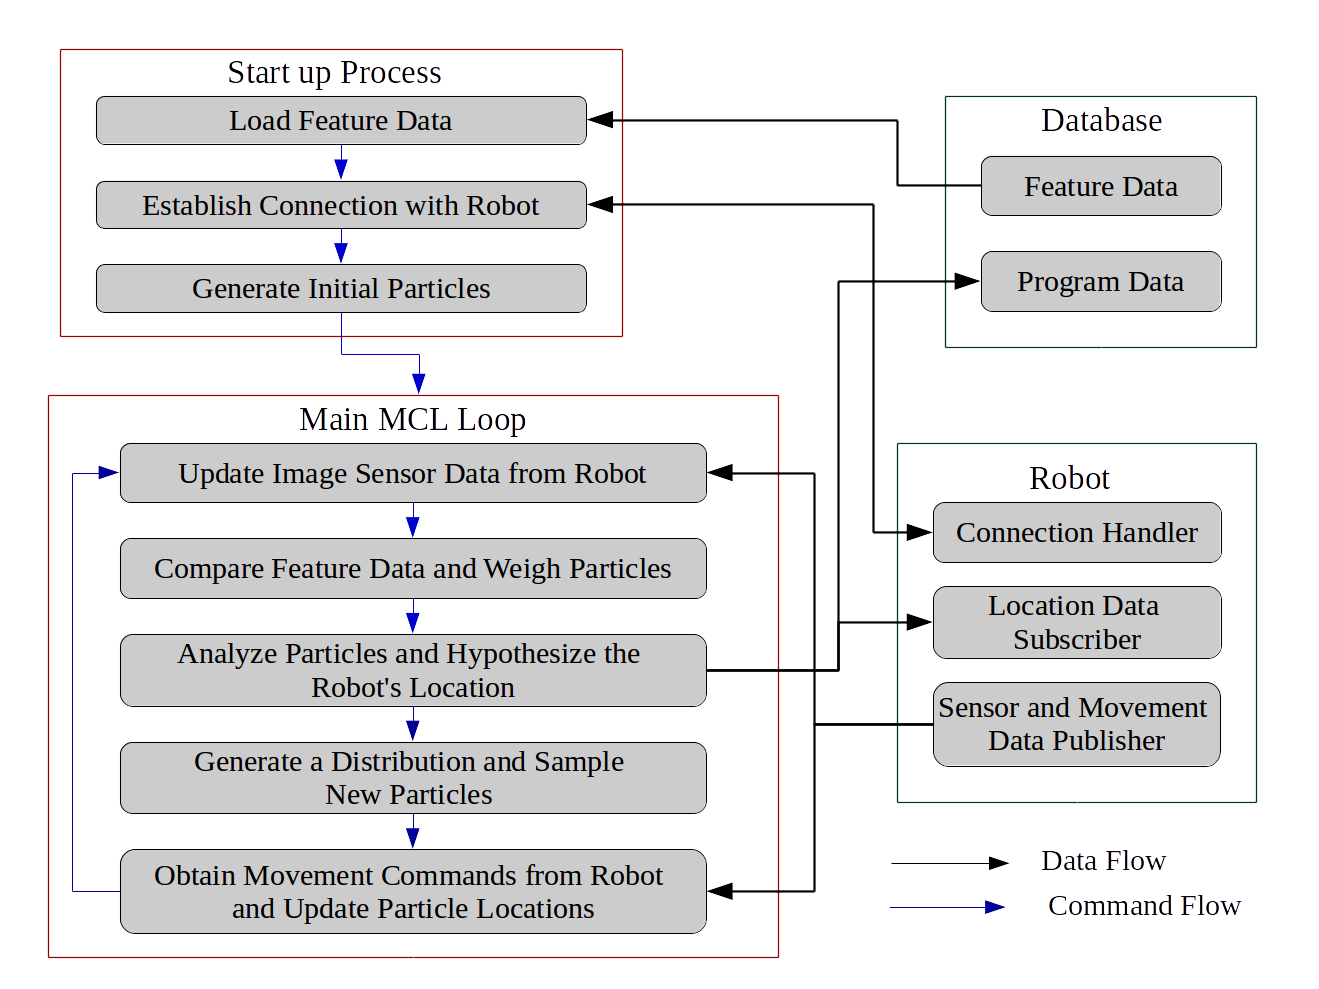
\includegraphics[width=\textwidth]{../Artifacts/FlowChart}
 \caption{Data and control flow of the 3DLocalization program}
\end{figure}


\subsection{Particle Generation}
\begin{itemize}
  \item \textbf{Generating a Distribution}
  \item \textbf{Sampling from the Distribution}
\end{itemize}

\subsection{Weighing the Particles}
Each particle in our particle vector contains a weight associated with it that represents the probability that the actor is currently at that particle's location in the real world. This weight is determined by comparing the precomputed feature data for the perspective associated with the particle to the feature data computed in real-time from the actor's image feed. The weight assigned to the particle will proportionally affect the probability of another particle being sampled from near that perspective in the environment during the next loop iteration of the algorithm.

Before a particle can be weighed, it must have its image features matched with the features from the actors image. This entails going through the features for both images and seeing which features match best to eachother. To begin, we will define what information is needed to start the feature matching process.
 \\ \\ 
  \[ \verb. Two vectors of SURF features. \] 
  \[ \boldsymbol{F_{robot}} \verb., . \boldsymbol{F_{particle}} \verb. where . \boldsymbol{F} = \verb. [. \mathtt{f_{1}} \verb., . \mathtt{f_{2}} \verb-, ... , - \mathtt{f_{n}} \verb. ]. \]
  \[ \verb. A distance function that compares two features. \]
 \[ f(\mathtt{[f_{pj}, f_{rk}]}) \to \mathtt{distance} \in \mathtt{R^+}\]

  % In its current implementation, our algorithm only uses SURF features to do the matching between image pairs. We set up the project to also do matching with SIFT and greyscale features, but these methods didn't seem to help our matching attemps so they are currently disabled.
   Our group decided to use an \texttt{OpenCV FlannMatcher} object to generate an initial matrix of matched features between the two images. The \texttt{FlannMatcher} object has a built-in function \emph{KnnMatch} that return a matrix of matching pairs. Each row of this matrix is a matching vector consisting of \texttt{n} columns, defines as follows.

 \[ \boldsymbol{m} = \mathtt{ [f_{j}} \verb., . \mathtt{f_{k1}} \verb., . \mathtt{f_{k2}} \verb-, ... ,- \mathtt{f_{kn}} ] \verb. such that . \]
 \[ f(\mathtt{[f_{j}, f_{k1}]}) < f(\mathtt{[f_{j}, f_{x}]}) \verb. . \forall \mathtt{ f_{x}} \in  \boldsymbol{F_r} \verb. . \]
 \[ f(\mathtt{[f_{j}, f_{k2}]}) < f(\mathtt{[f_{j}, f_{x}]}) \verb. . \forall \mathtt{ f_{x}} \in  [\boldsymbol{F_r} - \mathtt{f_{k1}]}  \verb, ... , \]
 \[ f(\mathtt{[f_{j}, f_{kn}]}) < f(\mathtt{[f_{j}, f_{x}]}) \verb. . \forall \mathtt{ f_{x}} \in  [\boldsymbol{F_r} - \mathtt{f_{k1} - \mathtt{f_{k2}} -} \verb,...,- \mathtt{f_{kn-1}}  ]  \verb. . \] 

 Thus a matching vector of length \texttt{n} contains a feature and the \texttt{n} features that are most similar to it. The \emph{KnnMatch} function of order \texttt{n} return a matrix with a matching vector of order \texttt{n} for each feature in both the robot and particle feature vectors. For our purposes, we ran the \emph{KnnMatch} function with \texttt{n = 2}. This gave us the two best matches for each feature.
 \[ Flann.KnnMatch(\boldsymbol{F_r} \verb., . \boldsymbol{F_p} \verb., . 2) \to \boldsymbol{M} = \mathtt{ [\boldsymbol{m}_0, \boldsymbol{m}_1, ... , \boldsymbol{m}_n ]} \]
 \[ \verb. Where . \boldsymbol{m_i} = \mathtt{ [f_{j}} \verb., . \mathtt{f_{k1}} \verb., . \mathtt{f_{k2}} ]\]

 The \emph{Flann} function will give us a matrix of feature matches, but these matches still need to be refined. the ratio test\footnote{See Lowe, David G. ``Distinctive Image Features from Scale-Invariant Keypoints." {\it International Journal of Computer Vision} (2004). pg 19-20.  \url{http://www.cs.ubc.ca/~lowe/keypoints/}.} we refine the matrix of top-two matches into a smaller vector of best matches. The ratio test is described below.
\\ \\
 \textbf{INSERT MATH HERE SHOWING THE RATIO TEST}
-\\
  Now we need to get some kind of score for how well the matches correspond to each other, and use this score to determine how closely the image from the actor and the image from the particle's perspective match with each other. Each pair of matching keypoints has a `distance` score that can be calculated. This value tells us roughly how similar that pair of keypoints are to one another. Using the vector of matching keypoint pairs, the overall weight for a particle is determined as follows

\[  \verb. Given a vector of . \mathtt{n} \verb. matching feature pairs. \]
\[  \boldsymbol{M} = \mathtt{ [\boldsymbol{m}_0, \boldsymbol{m}_1, ... , \boldsymbol{m}_n} ]  \verb. where . \boldsymbol{m_i} = \mathtt{ \mathtt{[f_{pi}, f_{ri}]} }   \]
\[  f(\boldsymbol{M}_i) \to \mathtt{distance} \in \mathtt{R^+}   \]
\[  \verb.Particle Weight . \mathtt{w} = \sum_{i=0}^{n} \frac 1{f(\boldsymbol{M}_i) + 0.8} \]

In summary, this algorithm iterates through all \texttt{n} pairs of keypoint matches in our vector of matches (\textbf{M}) and sum up a value that gets larger when the distance between the keypoints in an individual pair are small and smaller when that distance in large. The added 0.8 in the denominator is to stop a feature pair with a very low distance from having a disproportionally high influence on the overall weighting of the particle. For example,
\[ \verb.If . f(\boldsymbol{M}_i) \to \mathtt{distance} = \verb, 0.001 ., \]
Without the added contant (0.8) in the denominator
\[ \frac 1{f(\boldsymbol{M}_i)} = 1000\]

1000 is much too high of a value for a single match to contribute to the sum, so adding the extra contstant in the denominator makes it so even the best key point matches only add a value slightly greater than one to our sum. This algorithm possesses a few traits that are beneficial for the accuracy and speed of our program.
\begin{itemize}
  \item The value of the \texttt{w} variable increases as the number of keypoint matches increases. This is desired, an image pair with many feature matches has a higher chance of being them being similar images than an image pair with very few  feature matches.
  \item Keypoint pairs with a high distance (are not very alike) will contribute a small amount to the sum, while keypoints pairs with low distance (are quite similar) will contribute a larger amount to the sum. This will cause images with very similar keypoints to be weighted higher than images with non-similar keypoints.
\end{itemize}

Another formula that does well is the following:
\[
\mathtt{w} = \mathtt{n} - 10 \times \frac{\sum_{i}^{n} f(\boldsymbol{M}_i)}{\mathtt{n} + 1}
\]
This also rewards images that have many good matches with the first term, then penalizes pairs of images where the average match distance is high.

\subsection{Determining the Location}
The list of weighted particles has been computed and can now be used to locate the actor. There are a few ways the location can be determined: Top Match, Weighted Average, or a combination of the two. The Top Match is simply the perspective that has the highest weight. This is a fairly good estimate, however it disregards much of the information that the MCL algorithm provides, such as the weights of all other perspectives. 

The second option is the Weighted Average, which looks at the top $n$ particles (we used $n=20$). It finds the weighted average position of these particles and the most common orientation. This tends to be accurate, but can have problems when, for example, there is a region in the middle of a room that a actor cannot possibly be, it is possible to return a location inside this region. To combat this issue, we use the Top Match when the Weighted Average is at an impossible location.

\subsection{Visualization}
For the user to see how the localization program is working, various visualization assistants were constructed to accompany the program. A user is able to see what the robot sees, a top-down view of the map showing the location and relative weights of each particle, the Top Match and Weighted Average chosen by the program, and a three dimensional visualizer showing all the particles within the actual map.












\section{Results}
We can analyze how our program performs for each of the initial objectives.

\subsection{Runtime Speed}
Depending on the type of feature matching being performed and the number of particles currently active, our algorithm takes less than one second to determine a guess for the location of the actor. When the number of particles surpass 700, this time begins to noticeably take longer than a second. We consider the algorithm to be working in real time because it usually takes longer for the robot to make its move than the algorithm takes in each iteration.

\subsection{Accuracy}


\subsection{Versatility}
Our algorithm is versatile to the extent that a map exists. It works with any robot that communicates with ROS. As long as a map of an environment exists in .obj file format, the program is able to localize a stream of image data to the best of its ability.

\subsection{Ease of Use}%\begin{multicols}{2}















\section{Issues and Future Work}
\subsection{Dynamic Environments}
In our implementation we assume a static environment. This is not always the case, as there are often people inhabiting the same space as robots. Also, objects like chairs, coffee cups, and even tables are not guaranteed to remain in the same position for any period of time. Future work will involve locating objects that are deemed non-static and ignoring them in the weighing process. Moving objects, such as a person walking, ought to also be ignored.

\subsection{Wall Detection}
If the MCL program knew where walls are in the environment, smarter weighing and weeding procedures can be used. Knowledge of walls might allow a robot to decide which wall it is looking at within the map. Wall awareness also allows for the weeding-out of particles that pass through a wall during their movement process. Since a robot cannot pass through walls, the particle that moved through a wall is an impossible location, and ought to be removed from possible locations.

\subsection{Navigation}
It is certainly possible to implement a smarter navigation algorithm in which a robot knows where walls, doors, and tables are. In our current implementation the robot merely travels in a straight line from its location to the destination, however this can cause it to bump into tables or crash into walls. A smart navigation algorithm would allow the robot to pass through a door and, if it were a drone, to fly over tables.

\subsection{Weighing}
When each particle's image data is compared with that of the robot, there are many different ways to arrive at a similarity score. Currently we use only the number of feature matches and the ``goodness" of each match. There are, however ways to incorporate algorithms such as RANSAC (Random Sample Consensus) to consider how well the matches align with each other. In our attempts at using this strategy, however, we found it was difficult to find one formula that will consistently weigh pairs of images with different match quantities. In addition, there may be quick image comparison techniques available to relate the black and white and gray scale images.

\section{Conclusions}
What a dumb robot.








  








\end{document}